% IEEE Paper Template for US-LETTER Page Size (V1)
% Sample Conference Paper using IEEE LaTeX style file for US-LETTER pagesize.
% Copyright (C) 2006-2008 Causal Productions Pty Ltd.
% Permission is granted to distribute and revise this file provided that
% this header remains intact.
%
% REVISION HISTORY
% 20080211 changed some space characters in the title-author block
%
\documentclass[10pt,conference,letterpaper]{IEEEtran}
\usepackage{times,amsmath,epsfig}

\usepackage{subfigure}
\usepackage{color}
\usepackage{balance}  % for  \balance command ON LAST PAGE 
\usepackage{graphicx}
\usepackage{epstopdf}  % used for generating pdf 
\usepackage[english]{babel}
\usepackage[utf8]{inputenc}
\usepackage{amsmath}
\usepackage{graphicx}
\usepackage{caption}

\let\proof\relax
\let\endproof\relax
\usepackage{amsthm}


\usepackage{caption}
\usepackage{color}
\usepackage[ruled]{algorithm}
\usepackage{algorithmic}
\renewcommand{\algorithmiccomment}[1]{\bgroup #1 \egroup}
\usepackage{cite} % to sort cite 
\usepackage{multirow} % to use multirow 


\newcommand{\ie}[0]{\textit{i.e.}}
\newcommand{\eg}[0]{\textit{e.g.}}
\newcommand{\etal}[0]{\textit{et al.}}

\newcommand{\keobf}{\textit{$(k,\epsilon)$-obfuscation}}
\newcommand{\argmin}{\operatornamewithlimits{argmin}}
\newcommand{\norm}[1]{\left\lVert#1\right\rVert}
\newcommand{\repAn}[0]{\textnormal{Rep-An}}
\newcommand{\funcname}[0]{\textit{GenAnonymization}}

\theoremstyle{plain}
\newtheorem{theorem}{Theorem} 
\newtheorem{definition}{Definition}
\newtheorem{problem}{Problem}
\newtheorem{example}{Example}
\newtheorem{lemma}{Lemma}

\newcommand{\SysName}{Chameleon }
\newcommand{\SysNameNS}{Chameleon}

%
\title{Chameleon: Uncertain Graph Releasing Using Synthetic Private Uncertain Graph Models}

% \author{Dongqing Xiao,  Mohamed Y. Eltabakh, Xiangnan Kong \\ 
% \affaddr{Worcester Polytechnic Institute (WPI), Computer Science Department, MA, USA} \\
% \{dxiao,~meltabakh,~xkong\}~@wpi.edu}  
\author{%
% author names are typeset in 11pt, which is the default size in the author block
{Dongqing Xiao, Mohamed Y. Eltabakh, Xiangnan Kong}%
% add some space between author names and affils
\vspace{1.4mm}\\
\fontsize{10}{10}\selectfont\itshape
Computer Science Department, Worcester Polytechnic Institute \\
Worcester, United States of America\\
\fontsize{9}{9}\selectfont\ttfamily\upshape
\{dxiao,~meltabakh,~xkong\}~@wpi.edu\
}
\begin{document}
\maketitle


% NOTE keywords are not used for conference papers so do not populate them
% \begin{keywords}
% keyword-1, keyword-2, keyword-3
% \end{keywords}
%

\begin{abstract}  
Research on social and business applications requires open access to real datasets. Such datasets can be shared, generally in the form of uncertain graphs whose edges are labeled with a probability of existence. While releasing uncertain graphs often risks exposing sensitive user information to the public. Current works are based on deterministic graphs that overlook the inherent uncertainty in edges.
To overcome such limitation, our work seeks a solution to release \emph{uncertain graphs} with high utility while preserving privacy. 
\end{abstract}

\section{Introduction}

\label{sec:Intro}

% Graph-- Uncertain Graph--Examples 
Graphs are used to capture the complex relationships in emerging applications, such as business to business (B2B) and social networks. 
Sometimes, the existence of the relationship between two entities is uncertain. For instance, in social networks, nodes represents individual users, while edges represent friendship or trust link among them.  Usually, the link is derived by inference and prediction models built on interaction details~\cite{Lin_B2B,Adar_Managing_2007,Kempe_Maximizing_2003}. And, edge probability denotes the accuracy of a link prediction, or the trust of one person on another. 
In these applications, the data can be modeled and shared as uncertain graphs whose edges carries a probability of existence. The probability represents the confidence that the relationship holds in reality. 

\begin{figure}[!htb]
  \vspace{-7pt}
    \subfigure[Social Trust Network]{\label{fig:socialNetwork}
      \begin{minipage}[l]{0.46\columnwidth}
        \centering
        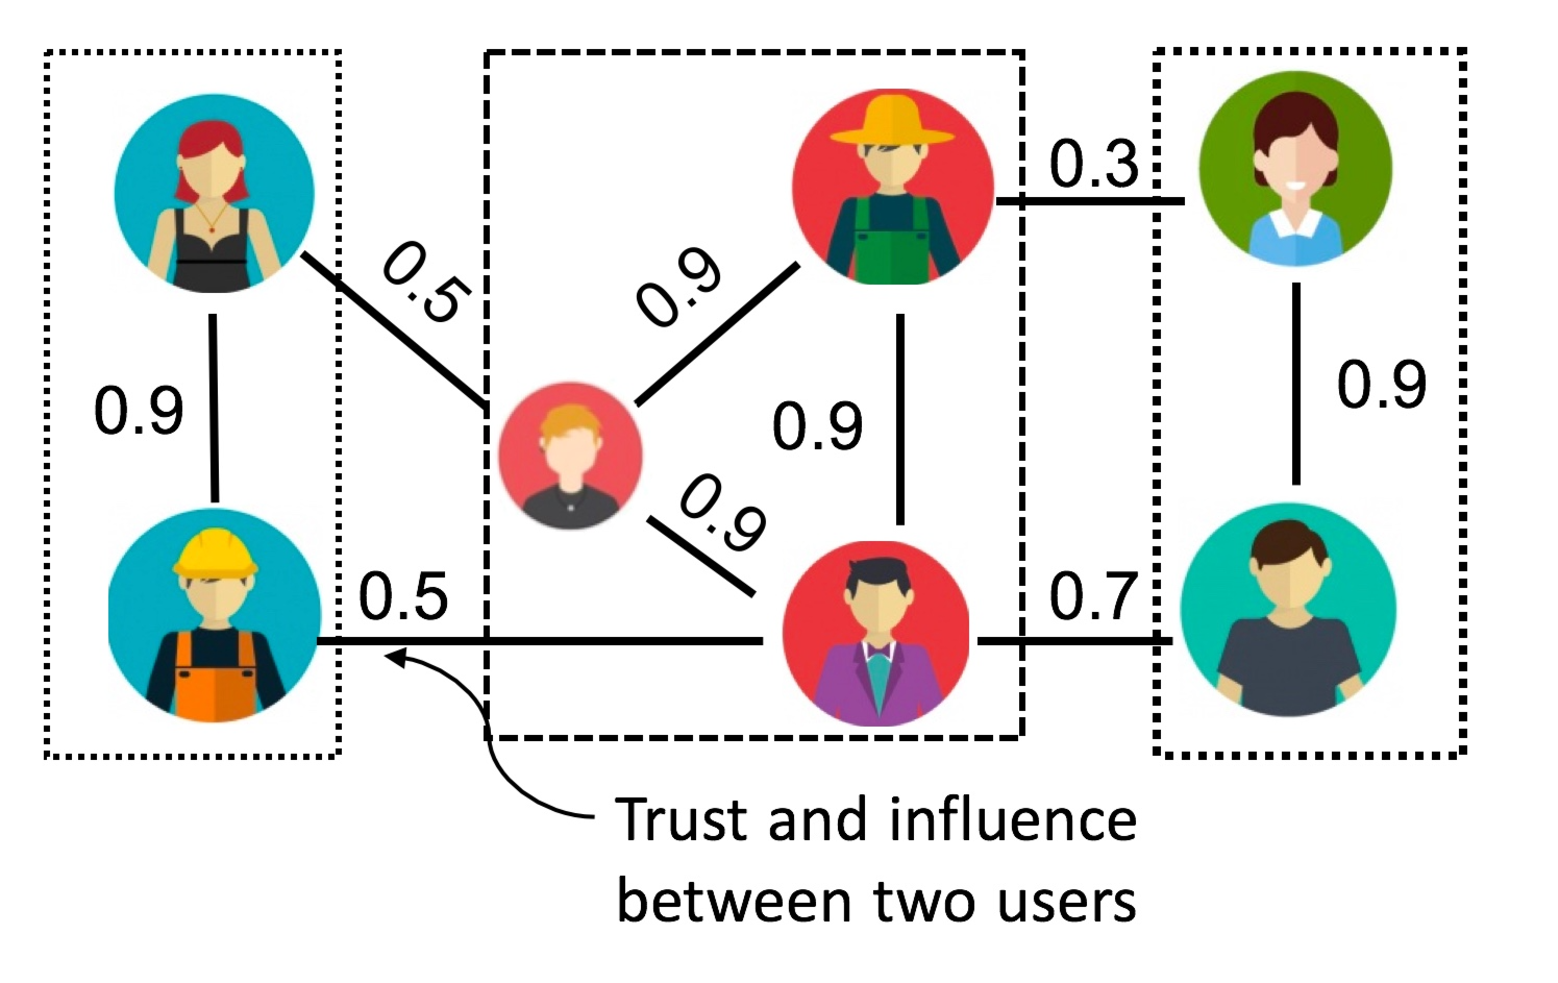
\includegraphics[height=2.7cm]{ill/SocialNetwork.pdf}
      \end{minipage}
      }
    \subfigure[B2B Network]{\label{fig:b2bNetwork}
      \begin{minipage}[l]{0.46\columnwidth}
        \centering
        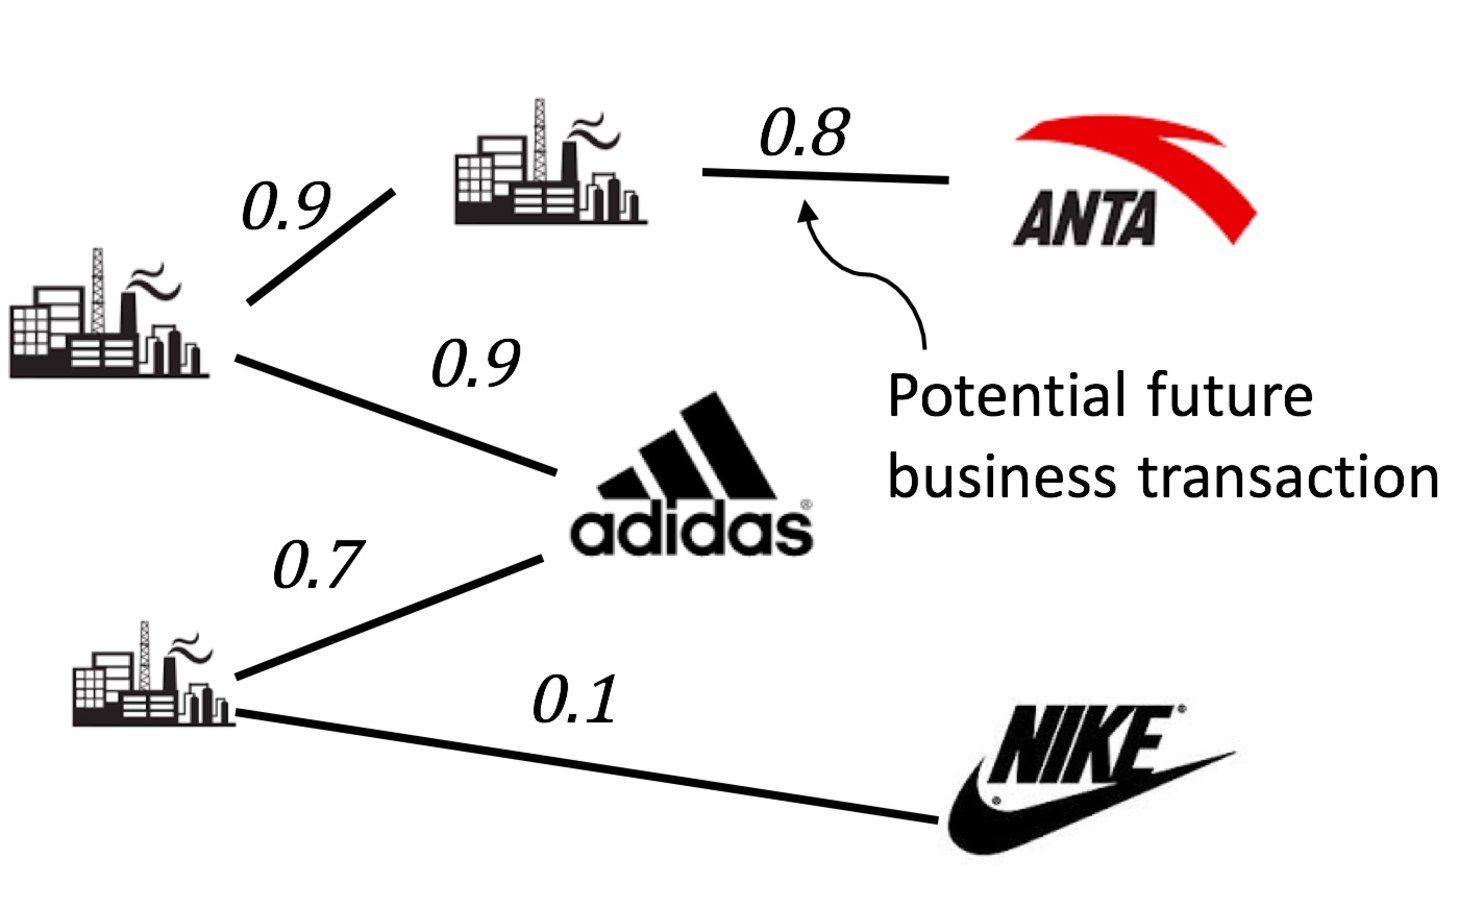
\includegraphics[height=2.7cm]{ill/B2BNetwork.pdf}
      \end{minipage}
      }
    \vspace{-7pt}
    \caption{Real-world uncertain graphs with privacy concerns.}
    \label{fig:motivation}
    \vspace{-7pt}
\end{figure} 

% Sharing--Privacy--Examples 
These uncertain graphs are invaluable for scientific research and commercial applications~\cite{Kempe_Maximizing_2003,Cho_Friendship_2011}. However, sharing these uncertain graphs would violate the privacy of users or entities profiled inside. In social trust network, the trust relationships among users--- which greatly impact users' behaviors, are usually probabilistic.  They are useful in social interaction study and micro-targeting. While users are unwilling to share such confidential information with potential adversaries like Cambridge Analytica. In B2B networks, business operators also hesitate to share transaction patterns as it relates to  confidential business models. Such tension is raising the question of sharing uncertain graphs without compromising privacy. 


% State-of-Art 
A number of privacy preserving graph sharing schemes have been studied in the deterministic scenario~\cite{Liu_Towards_2008,Ying_Randomizing_2008,Wang2011,Liu_Privacy_2009,Nguyen_Anonymizing_2015,Sala_Sharing_2011,Xiao_Differentially_2014,lee2011}, though many problems about sharing uncertain graphs still remain unexplored.  


An obvious approach is to convert uncertain graph sharing problem into the deterministic case by casting edge probabilities as edge weights. 
One of the most important goals of uncertain graph sharing is to maintain data utility. 
However, by disregarding the possible world semantics of the uncertain graph, such an approach fails to reflect uncertain graph properties such as connectivity, dense subgraphs correctly~\cite{Zhao_Detecting_2014,Hua_Probabilistic_2010}. {\small Note that connectivity of deterministic subgraphs is generally measured by the concept of cut, which is defined as the sum of weights of intra edges. Generally, the bigger the cut, the harder to separate two subgraphs. In Figure~\ref{fig:socialNetwork}, the equal cut $C(SG_{1},SG_{2})=C(SG_{3},SG_{2})=1$ implies the identical connectivity of $SG_{1}$ and $SG_{3}$ w.r.t $SG_{2}$. However, with the possible world semantics, we know the probability to separate $SG_{1}$ and $SG_{2}$ is $(1-0.5)^{2}=0.25$, and that to separate $SG_{2}$ and $SG_{3}$ is $(1-0.3)(1-0.7)=0.21$. Hence, in fact, $SG_{2}$ is closer to $SG_{1}$ than to $SG_{3}$.} 
Hence, the weighted graph anonymization scheme could produce very poor result in the uncertain scenario even if the anonymization algorithm is good.  


% Rep-OB 
Another approach, called by rep-based approach, is based on querying xxxx. 
As presented in our previous work~\cite{Xiao:2018}, it first extracts a single deterministic representative
instance $G$ that capture structural properties of the uncertain
graph.
After that, anonymization can be then be proceed efficiently on $G$ using conventional algorithms, regardless of the uncertainty.  
However, Rep-An is is not always feasible. 
The detachment of edge uncertainty deteriorates the data utility. 


As ever discussed, there is no utility guarntee in casting-based and rep-based approaches. 
Existing graph anonymization schemes are inadequate to share uncertain graphs with desirable trade-off between privacy and utility. 
There are the following distinct challenges in the uncertain scenario. 

$\bullet$~\textup{\emph{Stochastic Privacy Attacks.}}~~Edge uncertainty plays an indispensable role in the uncertain graph model. It is impractical to discard them in the release.  
While the extra release of edge uncertainty makes privacy protection far more difficult as it empowers the adversary and makes the profiled entity more vulnerable. 
% To this end, we show the potential re-identification attack and present the corresponding solution. 

$\bullet$~\textup{\emph{Stochastic Utility Loss Metric.}}~~It is very challenging to maintain the graph structure when the uncertain graph is modified to pursue anonymity. The structural distortion incurred is evaluated by the corresponding metric.  It plays the key role in utility preserving. Unfortunately, existing graph utility loss metrics such as graph edit distance~\cite{Liu_Towards_2008}, spectrum discrepancy~\cite{Ying_Randomizing_2008}, community reconstruction error~\cite{Wang2011} and shortest path discrepancy~\cite{Liu_Privacy_2009} are not suitable in the uncertain scenario because of the ignorance of edge probability. 
% In this context, the discrepancy w.r.t standard uncertain graph reliability becomes a good criterion. It evaluates the connectivity difference in the context of the entire graph and meanwhile utilizes the possible world model. 

$\bullet$~\textup{\emph{Intractable Search Space.}}~~It is very challenging to find a sanitized graph with the desired level of privacy by as few graph operations as possible. 
In the deterministic scenario, the problem is known to be NP-hard by edge additions and deletions~\cite{Hartung_Theory_2015}. 
In the uncertain scenario, the edge modification is no longer a binary operation (addition/deletion), but can be infinite probability values. Exhaustive search is computationally intractable if the number of edges is large.
 % Thus, we approximate the problem of interest via a randomized algorithm, which built on the basis of meta-heuristics. It excels in identifying a population of sanitized results with good quality.

In this work, we propose a solution tailored towards uncertain graphs via incorporating possible world semantics, {\methodName}. 
% {\methodName} is built on the basis of syntactic private notation. 
It preserves as much the stochastic nature of the original uncertain graph as possible, while injecting enough structural noise to guarantee a chosen level of privacy against re-identification attacks.
Specifically, we make the following contributions:
\begin{itemize}
\item To the best of our knowledge, we are the first to formulate the uncertain graph anonymization problem. 
 We show the potential re-identification attack and present the corresponding privacy notion. 
\item We propose an utility loss metric on the basis of generalized reliability. It evaluates the connectivity difference in the context of the entire graph and meanwhile utilizes the possible world model. 
\item We propose a randomized algorithm with dual meta-heuristics. By incorporating the possible world semantics, it excels in identifying a population of sanitized results with good quality.
\item We conduct extensive experimental studies to demonstrate efficiency and practical utility of our algorithms.
\end{itemize}

The rest of the paper is organized as follows. In Section 2, we summarize related works and clarify our distinct privacy goal. In Section 3 we formulate the uncertain graph-anonymization problem. Sections 4 – 5 consider the anonymization problem in the context of uncertain graphs.  In Section 6 we apply our method to several real-world uncertain graphs, and demonstrate their efficiency and practical utility. 


\section{Related Works}
A significant amount of prior work has been done protecting privacy of network datasets.
We summarize them here and clarify our privacy goals in this paper. 

\textbf{Graph Anonymization.}~ Early works on privacy-preserving network data publishing mainly focus on developing anonymization techniques for deterministic graphs against specific types of de-anonymization attacks. Most of them leverage privacy models derived from $k$-anonymity to create $k$ identical neighborhoods, or $k$ identical degree nodes. Current methods for anonymizing ``graphs" can be classified into four main categories: (1) Clustering-based generation~\cite{Hay_Anonymizing_2007,Bhagat_Class_2009,hay2010resisting}; (2)~{\em Edge modification}~\cite{Liu_Towards_2008, Zhou_Preserving_2008, Wang2011, Wu_k_2010, Skarkala_Privacy_2012}, 
(3)~{\em Edge randomization}~\cite{Liu_Privacy_2009,Ying_Randomizing_2008, Ninggal_Utility_2015},
and~(4)~{\em Uncertainty semantic-based modifications} which add uncertainty to some edges and thus converting the graph to an uncertain version~\cite{Boldi_Injecting_2012, Nguyen_Anonymizing_2015}. 
The uncertainty semantic-based approaches transform the original determinitic graph into an uncertain one to be published. These techniques are known as the state-of-art for their excellent privacy-utiltiy tradeoff brought by the fine-grained pertubation leveraging the uncertain semantics. As ever mentioned, these techniques are tailored to determinitic graphs (unweighted \& weighted). In this work, we further explore the privacy preserving problem in uncertain graph publication. 


\textbf{Diffiential Privacy.}~ The recent research on applying differential privacy to network data roughly falls into two directions. The first direction aims to release certain differentially private data mining results, such as degree distributions, sub-graph counts and frequent graph patterns. Such methods that release only query results require tracking tracking the results: early uses of the data can effect the quality of later uses, thus no new queries can be permitted on the data.  
The second direction aims to publish a sanitized graph. Most research in this direction projects an input graph to dK-series and ensures differential privacy on dK-series statistics. These private statistics are then either fed into generators or MCMC process to generate a fit synthetic graphs. While, current techniques are still inadequate to provide desirable data utility for many graph mining tasks. 



\textbf{Our Goals:Privacy Model \& Data Model}~
$\epsilon$-differential privacy does relate to individual identifiability and provide strong privacy guarntee without making any assumption of privacy risks. While, the privacy parameter $\epsilon$ does not have such a clear relation. There is no clear way to set a general policy for a value $\epsilon$ that provides sufficient privacy. In constrast to $\epsilon$-differential privacy, syntactic privacy model can generally be defined and understood based on the data schema; parameters have a clear privacy meaning that can be understood independent of the actual data and have a clear relationship to the legal concept of individual identifiability of data~\cite{}.  

Our general approach is to produce synthetic graphs by adding controlled perturbations to the structure of the original \emph{uncertain graph}. The generic approach can provide protection against identity disclosure and link disclosure. The choice directly impacts how much structural noise must be introduced to obtain a given level of privacy guarantees. In this paper, we chose to target against node re-identification problem for {\emph uncertain graph} releasing because . 
\section{Problem Definition}
\label{sec:notation}

In this section, we present the notations, definitions and the problem formulation.  
% In this section, we present the models of uncertain graph, privacy criteria, and utility metric. We then present the formal formulation of 
% uncertain graph anonymization problem. 

\subsection{Uncertain Graph}
% Let $\mathcal{G}=(V,E,\mathit{p})$ be an uncertain graph, where $V$ is the set of nodes, $E$ is the set of edges, and function $\mathit{p}: E \rightarrow [0,1]$ assigns a  probability of existence to each edge, denoted as $\mathit{p}(e)$. 
An uncertain graph $\mathcal{G}=(V,E,\mathit{p})$, is defined over a set of nodes $V$, a set of edges $E$, and a set of probabilities $\mathit{p}$ of edge existence. Following the literature, we consider the edge probabilities independent~\cite{Potamias_K_2010,Zhao_Detecting_2014,Jin_Distance_2011}, and we assume \emph{possible-worlds} semantics~\cite{Colbourn_Colbourn_1987}. Specifically, the \emph{possible world} semantics interprets $\mathcal{G}$ as a set of possible deterministic graphs 
$W(\mathcal{G}) = \{G_1, G_2, ..., G_n\}$, where each deterministic graph $G_i \in W(\mathcal{G})$ includes all vertices of $\mathcal{G}$ 
and a subset of edges $E_{G_i} \subset E$.  
The probability of observing any possible world $G_i=(V,E_{G_i}) \in W(\mathcal{G})$ is    
\begin{equation*}
    Pr[G_i]=\prod_{e \in E_{G_i}} {\mathit{p}(e)} \prod_{e \in E \setminus E_{G_i}} (1-\mathit{p}(e))
\end{equation*}

In this work, we assume the input uncertain graph undirected and contains no self-loops or multiple edges. 


\subsection{Reliability-Based Utility Loss Metric}
A well-chosen utility-loss metric may lead to substantially less sanitized graphs at a minimal loss of information. 
As be known to all, connectivity is a fundamental graph property and plays an important role in graph mining tasks such as locating $k-$nearest neighbor~\cite{Potamias_K_2010}, graph clustering~\cite{Asthana_Predicting_2004} and shortest paths detecting~\cite{Zhao_Detecting_2014}. Moreover, the connectivity model has been shown to be able to yield better representation than degree sequence model. The connectivity discrepancy was proven to be a proper utility-loss metric. Therefore, we use its generalized version -- Reliability Discrepancy as the utility-loss metric in the uncertain graph context. 
 
In uncertain graphs, the concept of reliability is used to generalize \emph{connectivity} by  capturing the probability that two given (sets of) nodes are reachable over all possible worlds of the uncertain graph as follows:
\begin{definition}
    \textbf{Two-Terminal Reliability~\cite{Colbourn_Colbourn_1987}}  Given an uncertain graph $\mathcal{G}$, and two distinct nodes $u$ and $v$  $\in~V$, the reliability of $(u,v)$ is defined as:
        \begin{equation*}
                R_{u,v}(\mathcal{G})= \sum_{G \in W(\mathcal{G})}  \mathcal{I}_{G}(u,v) Pr[G] 
        \end{equation*}
    where $\mathcal{I}_{G}(u,v)$ is 1 iff $u$ and $v$ are contained in a connected component in $G$, and 0 otherwise.   
    \label{d:reliability}
\end{definition}


\theoremstyle{definition}
\begin{definition}
    \textbf{Graph Reliability Discrepancy}
    The reliability discrepancy of graph $\tilde{\mathcal{G}}=(V,E, \tilde{\mathit{p}})$, 
    denoted as $\Delta(\tilde{\mathcal{G}})$, 
    w.r.t. an original graph  $\mathcal{G}=(V,E,\mathit{p})$  is 
    defined as the sum of the two-terminal reliability discrepancy over all node pair $(u,v) \in V_\mathcal{G}$.
    \begin{equation*}
        \Delta(\tilde{\mathcal{G}})=\sum_{(u,v) \in V_\mathcal{G} }|R_{u,v}(\mathcal{G})-R_{u,v}(\tilde{\mathcal{G}})|
    \end{equation*}
\end{definition}


\subsection{Attack Model and Privacy Criteria}
\label{sec:AMPC}
In this paper, we focus on the ``identity disclosure problem"~\cite{Liu_Towards_2008} over uncertain graphs, which is one serious privacy leak concern when a graph dataset is published. Formally, give a published graph $G$, if and adversary can locate the target entity $t$ as a vertex $v$ of $G$ with a high probability via auxiliary information, we said that the identity of $t$ is disclosed. The popular assumption of auxiliary information is node degree~\cite{Liu_Towards_2008}. 

Following the literature, we adopt the syntactic $\keobf$ criterion~\cite{Boldi_Injecting_2012} for privacy guarantee. 
Analogous to the well known $k$-anonymity notion, $k$-obf requires to blend every vertex with \emph{other} fuzzy-matching nodes. 
Compared to $k$-anonymity, $k$-obf, which is global and entropy-based quantification, is more adequate than the previous used local quantification based on a posteriori belief probabilities. An excellent discussion on $k$-obf was presented by Bonchi {\etal}~\cite{Bonchi_Identity_2014}. 
Moreover, the introduction of a tolerance parameter $\epsilon$, which allows skipping up to $\epsilon * |V|$ nodes, makes it more practical. The skipped nodes might be extreme unique nodes, e.g., Trump in a Twitter network, whose obfuscation is almost impossible.
The formal definition is as follows:
\theoremstyle{definition}
\begin{definition}
	\textbf{\boldmath{$(k,\epsilon)$}-obf \cite{Boldi_Injecting_2012}}
    Let $P$ be a vertex property (i.e., vertex degree in our work), $k \geq 1$ be a desired level of anonymity, and $\epsilon >0 $ be a tolerance parameter. 
    An sanitized uncertain graph $\tilde{\mathcal{G}}$ is said to $k$-obfuscate a given vertex $v \in \mathcal{G}$ w.r.t $P$ if the entropy $H()$ of the distribution $Y_{P(v)}$ over the nodes 
    of $\tilde{\mathcal{G}}$ is greater than or equals to $\log_{2}{k}$:
    \begin{equation*}
        H(Y_{P(v)}) \geq \log_{2}{k}.
    \label{obfCon}
    \end{equation*}
The uncertain graph $\tilde{\mathcal{G}}$
is $(k,\epsilon)$-obf w.r.t property $P$ 
if it $k$-obfuscates at least $(1-\epsilon)|V|$ nodes in $\mathcal{G}$. 
\label{def:obf}
\end{definition} 

\subsection{Problem Statement}
% add one sentence to address this one 
Given the above foundation, we can now formulate the addressed problem.  
\begin{problem}
	\textbf{Reliability-Preserving Uncertain Graph Anonymization}
     Given an uncertain graph $\mathcal{G}=(V,E,\mathit{p})$ and anonymization parameters $k$ and $\epsilon$, 
     the objective is to find a  $(k,\epsilon)$-obfuscated uncertain graph $\tilde{\mathcal{G}}=(V,E,\tilde{\mathit{p}})$ 
     with minimal  $\Delta(\tilde{\mathcal{G}})$. That is:
     \begin{equation*}
             \begin{aligned}
                 & \argmin_{\tilde{
                \mathcal{G}}} & & \Delta(\tilde{\mathcal{G}}) \\
                &  \text{Subject to} & &\tilde{\mathcal{G}} \text{~is~} (k,\epsilon)-obf
            \end{aligned}
     \end{equation*}
     \label{prob:unobf}
\end{problem}
\section{The Representative Anonymization Algorithm}
\label{sec:repOB}
Instead of designing new methods for \emph{uncertain} graphs, we first consider somehow utilizes methods for deterministic graphs. Fortunately, there has been extensive work on extracting a single representative instance (deterministic one) of uncertain graphs that capturing graph statistics such as the expected vertex degrees~\cite{Parchas_Gullo_Papadias_Bonchi_2014}.  

Motivated by the preceding, in this work we introduce the representative anonymization (Rep-An) algorithm that combines isolated but complementary work from literature for uncertain graph anonymization. As shown in Figure\ref{fig:repOB}, we first extract a single \emph{representative} instance from an original uncertain graph. Then, conventional anonymization techniques can be then applied on this representative to attain closely approximate anonymized output of the original uncertain graph. This body of research comes to its aid that anonymization can be carried out on uncertain graphs, regardless of the uncertainty inherent in the data.


However, this approach has several limitations. First, the input edge uncertainties (probabilities) are no longer integrated into the anonymization process since they are detached from the graph in the first step. Second, the anonymization process (the second step) is oblivious to the {\em reliability} metric since its input is a made-up deterministic graph. Third, since the two phases are isolated from each other, different phases are optimized for different metrics. As the result, this naive \texttt{Rep-An} approach introduces a high level of noise and consequently deteriorates the overall utility of the anonymized graph. 
In the experiment section, we further study this approach empirically and confirm its impracticality.

\begin{figure}[t]
	\vspace{-1em}
    \captionsetup{margin=0cm}
    \centering  
        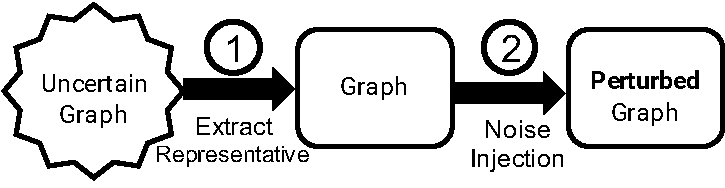
\includegraphics[width=0.95\columnwidth]{AddFigure/repOB.pdf}
        \vspace{-0.7em}
    	\caption{Overview of Rep-An. Noise is added to the extracted \emph{representative} instance.}
    \label{fig:repOB}
    \vspace{-0.5em}
\end{figure}
\subsection{Validation on Real Uncertain Graphs}
In this section, we empirically evaluate the impact of noise injected to extracted \emph{representative} instances by executing Rep-An on real uncertain graphs.

\textbf{Uncertain Graphs.}~~We use three uncertain graphs that capture different real-world scenarios and have been used in prior uncertain graph mining studies. Table~\ref{tab:dataset} lists uncertain graphs and their tolerance parameters used in our evaluation.

\textsc{DBLP} is a co-authorship network where the probability of an edge between two authors represents the likelihood two authors will collaborate in the future. The probability is obtained by a predictive model based on historical co-authorship data.~\cite{Jin_Distance_2011}. 

\textsc{Brightkite} is a location-based social network where the probability of an edge between two users corresponds to the chance that two users visit each other. The probability can be obtained by a prediction model based on historical data~\cite{Cho_Friendship_2011}.

\textsc{PPI} is a dataset of protein-protein interactions, provided by Disease Module Identification DREAM Challenge, where the probability of any edge corresponds to the confidence that the interaction actually exists.
The probability is obtained through biological experiments.

% Add one sentence 
\begin{table}[t]
    \centering
        \caption{Characteristics of the datasets and privacy parameters}
        \begin{tabular}{|c|c|c|c||c|}
        \hline 
        Graph    & Nodes    & Edges    &Edge Prob    & Tolerance level\\
        \hline  
        DBLP     &824,774   &5,566,096 & 0.46        & $10^{-4}$\\
        \small{BRIGHTKITE} &58,228   & 214,078 &0.29 &$10^{-3}$ \\
        PPI      &12,420   & 397,309  & 0.29         &$10^{-2}$\\
        \hline
        \end{tabular}
        \label{tab:dataset}
\end{table}

\begin{figure}[!htb]
  \subfigure[\small Edge Probability Distribution]{\label{subfig:edgepro}  
    \begin{minipage}[l]{1\columnwidth}
      \centering
       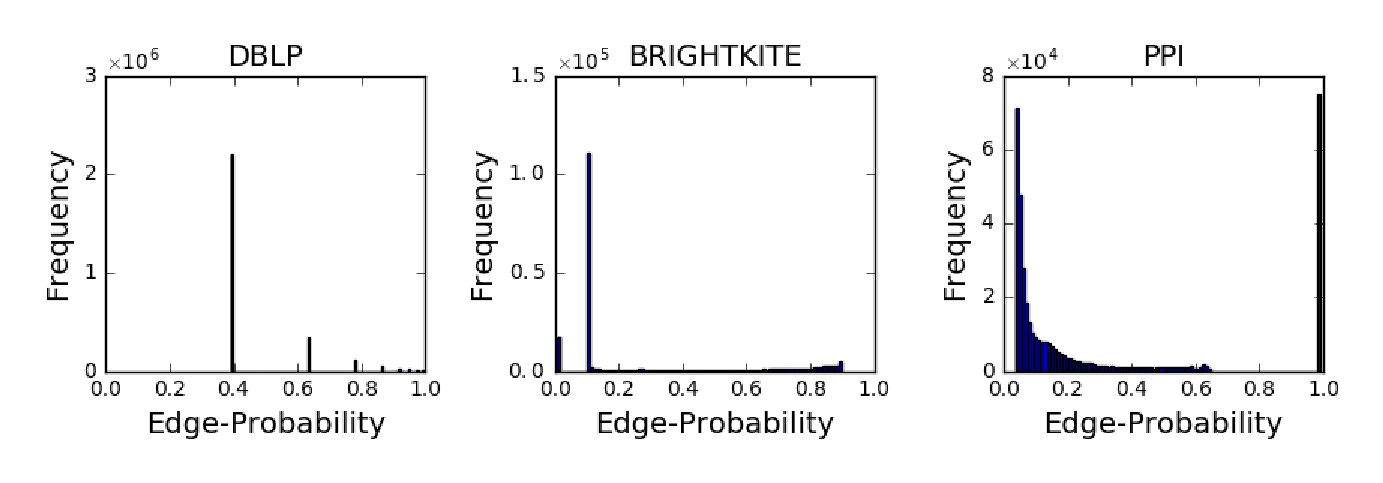
\includegraphics[width=\linewidth]{exp/edge_prob_row.eps}
    \end{minipage}
    \vspace{-15pt}
  }
  \subfigure[\small Expected Degree Distribution]{\label{subfig:degreepro}  
    \begin{minipage}[l]{1\columnwidth}
      \centering
       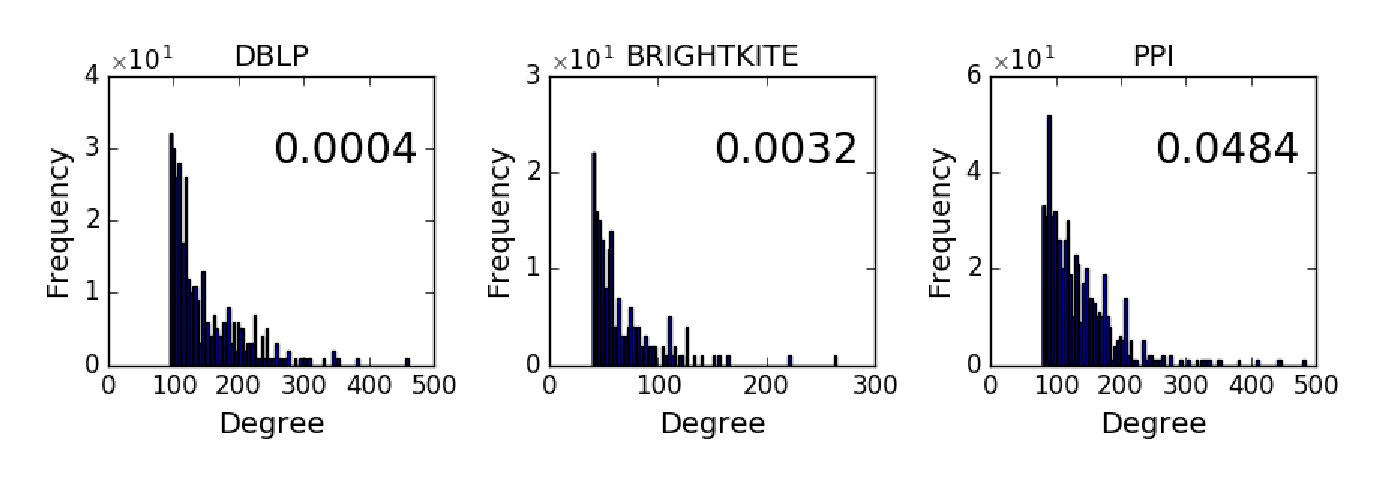
\includegraphics[width=\linewidth]{exp/degree_row.eps}
    \end{minipage}
  }
    \vspace{-10pt}
    \caption{Edge probability\& degree distributions.}
    \label{fig:summary_graph}
   \vspace{-15pt}
\end{figure}

Figure~\ref{subfig:edgepro} shows the edge-probability distribution in the three datasets. 
Note that the DBLP dataset only has  a few probability values, while Brightkite dataset's probability values are generally very small.The PPI dataset has a more uniform probability distribution. 
We also present their degree distributions of ``unique'' nodes (with high degree and obfuscation level is smaller than $300$). Observe that, all the three graphs have a heavy-tailed degree distribution (i.e, an amount of ``unique" nodes). In the context of graph privacy, the larger amount of ``unique'' nodes requires a larger amount of noise.


% pass 
\textbf{Computation.}~~We extract the single representative instances for each uncertain graph, introduce noise using the state-of-art graph anonymization strategy, and then compute the Reliability Discrepancy between the perturbed graph and the original uncertain graph as a measure of the level of graph structural error introduced. We approximate its expectation value by the average value obtained over the sampled possible worlds. Here, we use 1,000 samples since it has been shown that $1000$ usually suffices to achieve accuracy converge~\cite{Potamias_K_2010}.

\textbf{Results.}~~Figure~\ref{} shows that the Rep-An algorithm produces a large error for large values of $k$ (i.e. strong privacy guarntees). As we mentioned, the low level of utility is due to the large noise Rep-An injects into the representative instance, resulting in a perturbed graph (uncertain one) which is significantly different from the original \emph{uncertain} graph. 

The high discrepancy is largely due to the representative extraction step. In the extreme case where $k=1$ (i.e. no privacy guarntees), the sole representative extraction step produces high reliability errors. 
To better understand its limitation, we report the potential lower-bound on the error that could be achieved via Chamelon methods in Figure~\ref{}. Indeed, Figure~\ref{} shows that the utility loss of the Rep-An strategy can largely be attributed to the overlook of edge uncertainty.   
% add one sentence about the
% add more sentences to highlight their difference. 





\bibliographystyle{abbrv}
\bibliography{refs}

\end{document}
